\section{Model Adaptiveness Evaluation}
\label{sec:model_adaptiveness}

To evaluate how well our Q-table model generalizes to unseen data distributions, we conducted experiments using Gray-Scott reaction-diffusion simulation data. The Gray-Scott system produces structured spatiotemporal patterns with characteristics distinct from our synthetic training distributions, making it an ideal test case for model adaptiveness. We simulated 8 parallel process configurations with grid size $L=384$, generating 16 test data chunks (U and V concentration fields) representing diverse pattern types including spots, stripes, coral, and mitosis formations.

The initial Q-table achieved 50\% state coverage on Gray-Scott data out of the box, with the remaining states falling back to global averages. While this demonstrates reasonable generalization, the initial predictions were poorly calibrated---the model predicted compression ratios of 180--691$\times$ when actual values were 18--23$\times$, reflecting the fundamental difference between synthetic training data and real scientific simulation patterns. This motivates the use of online reinforcement learning to adapt the model to deployment-specific data characteristics.

We evaluated the Q-table's adaptation capability over 40 reinforcement learning iterations, measuring two complementary metrics: Mean Absolute Percentage Error (MAPE) for absolute prediction accuracy, and Kendall's $\tau$ for ranking correlation. Each iteration tested 11 compressor configurations across the 16 data chunks, with Q-values updated using a learning rate of $\alpha = 0.3$. Figures~\ref{fig:mape} and~\ref{fig:kendall_tau} show the evolution of these metrics for three prediction targets: compression ratio, compression time, and decompression time.

\begin{figure}[htbp]
\centering
\includegraphics[width=0.85\textwidth]{gray_scott_mape.pdf}
\caption{Mean Absolute Percentage Error over reinforcement learning iterations. Compression ratio MAPE drops from 689.8\% to 83.6\% within the first few iterations (initial value annotated as it exceeds the 150\% axis limit). Compression and decompression time predictions remain relatively stable, with decompression time improving from 35\% to 23\%.}
\label{fig:mape}
\end{figure}

\begin{figure}[htbp]
\centering
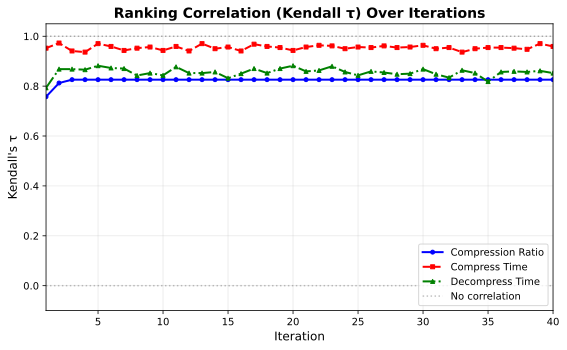
\includegraphics[width=0.85\textwidth]{gray_scott_kendall_tau.pdf}
\caption{Kendall's $\tau$ ranking correlation over reinforcement learning iterations. Compression time ranking achieves near-perfect correlation ($\tau > 0.95$) from the first iteration. Compression ratio and decompression time rankings improve steadily, reaching $\tau = 0.83$ and $\tau = 0.85$ respectively by iteration 40.}
\label{fig:kendall_tau}
\end{figure}

The results reveal distinct learning patterns for each target. Compression ratio shows the most dramatic improvement, with MAPE dropping 8$\times$ within the first 5 iterations as the Q-table learns that Gray-Scott data achieves different ratios than synthetic training data. Compression time predictions are already well-calibrated from the start, achieving Kendall's $\tau > 0.95$ immediately---indicating that timing knowledge transfers effectively across data distributions. Decompression time improves steadily throughout training, with MAPE dropping from 35\% to 23\% and ranking correlation increasing from 0.79 to 0.85.

The high Kendall's $\tau$ values are particularly significant for practical compressor selection. Even when absolute predictions have residual error, the model correctly identifies which compressors are faster or slower and which achieve better or worse compression ratios. This enables optimal selection decisions based on relative performance ranking rather than absolute values. The Q-table converges within approximately 880 compression operations (5 iterations), demonstrating that online learning can rapidly adapt the model to any deployment environment. This transforms the Q-table from a static model requiring representative training data into a dynamic system suitable for diverse scenarios including scientific computing, where data characteristics may differ substantially from typical training distributions.
